
\tikzset{every picture/.style={line width=0.75pt}} %set default line width to 0.75pt        

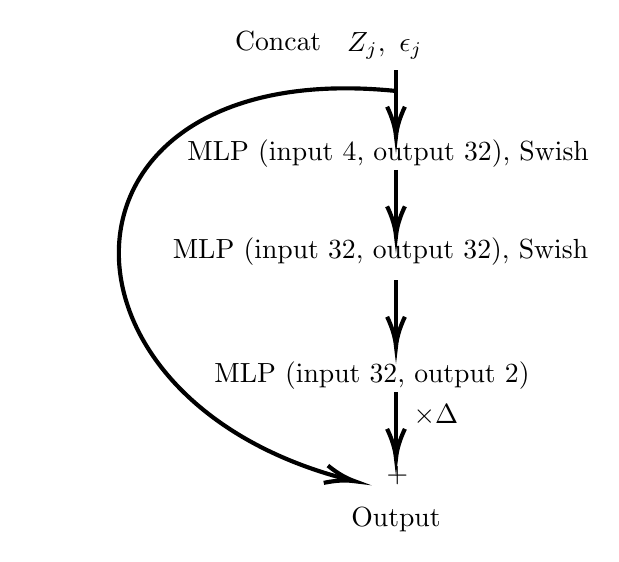
\begin{tikzpicture}[x=0.75pt,y=0.75pt,yscale=-1,xscale=1]
%uncomment if require: \path (0,300); %set diagram left start at 0, and has height of 300

%Straight Lines [id:da5030556769201339] 
\draw [line width=1.5]    (140,22) -- (140,50.8) ;
\draw [shift={(140,53.8)}, rotate = 270] [color={rgb, 255:red, 0; green, 0; blue, 0 }  ][line width=1.5]    (14.21,-4.28) .. controls (9.04,-1.82) and (4.3,-0.39) .. (0,0) .. controls (4.3,0.39) and (9.04,1.82) .. (14.21,4.28)   ;
%Straight Lines [id:da34385996465023216] 
\draw [line width=1.5]    (140,70) -- (140,98.8) ;
\draw [shift={(140,101.8)}, rotate = 270] [color={rgb, 255:red, 0; green, 0; blue, 0 }  ][line width=1.5]    (14.21,-4.28) .. controls (9.04,-1.82) and (4.3,-0.39) .. (0,0) .. controls (4.3,0.39) and (9.04,1.82) .. (14.21,4.28)   ;
%Straight Lines [id:da04663118080544015] 
\draw [line width=1.5]    (140,177.2) -- (140,206) ;
\draw [shift={(140,209)}, rotate = 270] [color={rgb, 255:red, 0; green, 0; blue, 0 }  ][line width=1.5]    (14.21,-4.28) .. controls (9.04,-1.82) and (4.3,-0.39) .. (0,0) .. controls (4.3,0.39) and (9.04,1.82) .. (14.21,4.28)   ;
%Curve Lines [id:da49947456616582553] 
\draw [line width=1.5]    (140,32) .. controls (-31.64,14.59) and (-36.46,180.33) .. (117.66,219.42) ;
\draw [shift={(120,220)}, rotate = 193.65] [color={rgb, 255:red, 0; green, 0; blue, 0 }  ][line width=1.5]    (14.21,-4.28) .. controls (9.04,-1.82) and (4.3,-0.39) .. (0,0) .. controls (4.3,0.39) and (9.04,1.82) .. (14.21,4.28)   ;
%Straight Lines [id:da0901728238287568] 
\draw [line width=1.5]    (140,123.2) -- (140,152) ;
\draw [shift={(140,155)}, rotate = 270] [color={rgb, 255:red, 0; green, 0; blue, 0 }  ][line width=1.5]    (14.21,-4.28) .. controls (9.04,-1.82) and (4.3,-0.39) .. (0,0) .. controls (4.3,0.39) and (9.04,1.82) .. (14.21,4.28)   ;

% Text Node
\draw (115,2.4) node [anchor=north west][inner sep=0.75pt]    {$Z_{j} ,\ \epsilon _{j}$};
% Text Node
\draw (38,54) node [anchor=north west][inner sep=0.75pt]   [align=left] {MLP (input 4, output 32), Swish};
% Text Node
\draw (51,161) node [anchor=north west][inner sep=0.75pt]   [align=left] {MLP (input 32, output 2)};
% Text Node
\draw (147,181.4) node [anchor=north west][inner sep=0.75pt]    {$\times \Delta $};
% Text Node
\draw (134,211.4) node [anchor=north west][inner sep=0.75pt]    {$+$};
% Text Node
\draw (117,231) node [anchor=north west][inner sep=0.75pt]   [align=left] {Output};
% Text Node
\draw (31,101) node [anchor=north west][inner sep=0.75pt]   [align=left] {MLP (input 32, output 32), Swish};
% Text Node
\draw (61,2) node [anchor=north west][inner sep=0.75pt]   [align=left] {Concat};

\end{tikzpicture}